% Provenance (never printed): cycle 4 SVT, "La planete Terre": volcanic
% activity, its products and its link with plate boundaries; natural hazards
% and their monitoring; see sources/book1/PROVENANCE.md. Book 1, grade 7,
% chapter 2.
% Vocabulary guard: "magma" first allowed here; "sediment" not before g7.4;
% "subduction zone" is never a term here (gloss: "where one plate sinks under
% another"); "hotspot track" is Book 2's; lahars are called mudflows.
\chapter{火山}\label{ch:g7:volcanoes}

1980 年 5 月 17 日，一位地质学家站在距美国西北部圣海伦\omterm{def:g4:volcanoes-earthquakes-first-look:volcano}{火山} 10 千米的山脊上，
拍下了下方左图：一座光滑的、覆盖着积雪的圆锥形山峰，
是美国最优美的山峰之一。
两个月来，这座山一直在颤动，
它的北侧像气球一样向外鼓起。第二天早上，
8:32，一次小\omterm{def:g4:volcanoes-earthquakes-first-look:earthquake}{地震}使它震动。整个隆起的北侧滑落下去，
\omterm{def:g4:volcanoes-earthquakes-first-look:volcano}{火山}向侧面爆发。同一山脊于
9 月再次拍照时，这座山的样子如右图所示。

\begin{omfigure}
\begin{minipage}[b]{0.495\linewidth}\centering
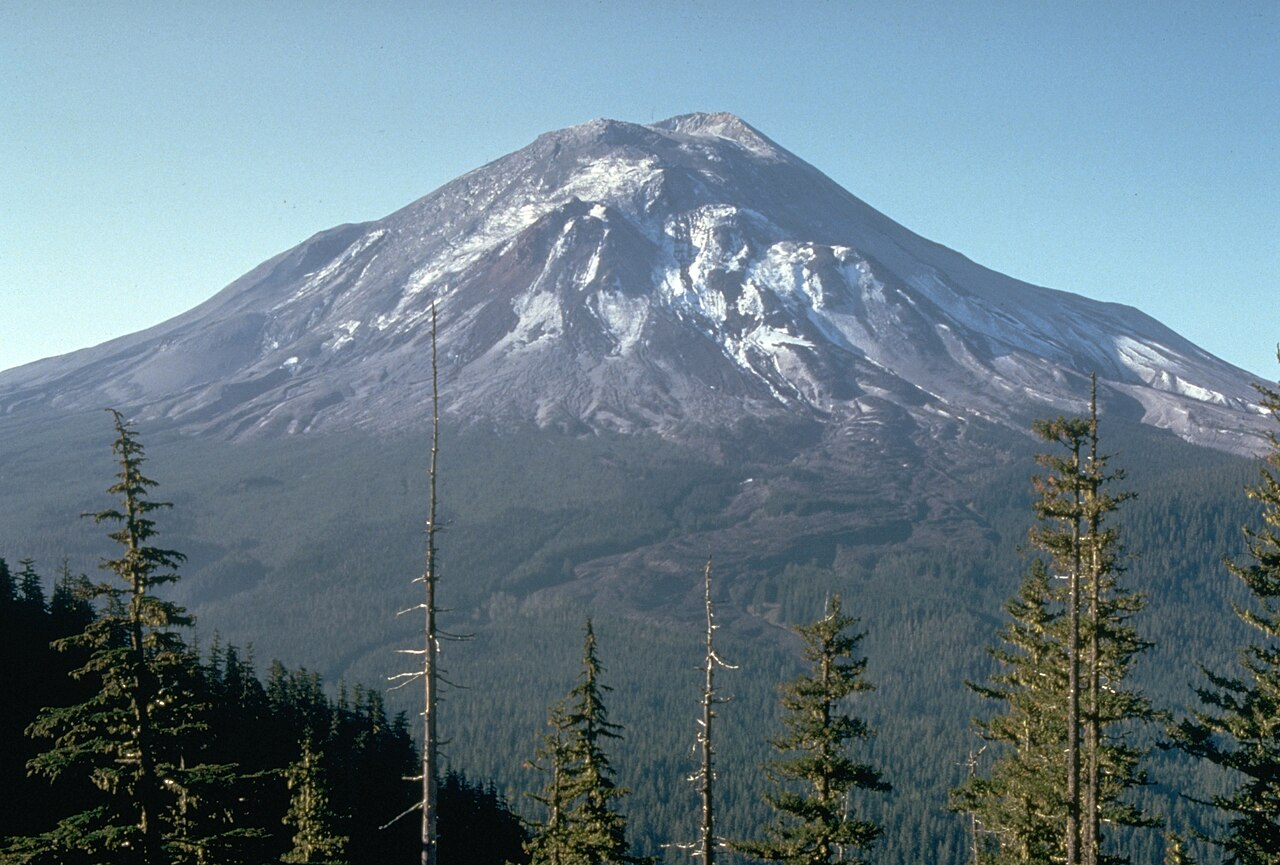
\includegraphics[width=\linewidth]{images/book1/g7-msh-before.jpg}

{\small 1980 年 5 月 17 日，爆发前一天。}
\end{minipage}\hfill
\begin{minipage}[b]{0.495\linewidth}\centering
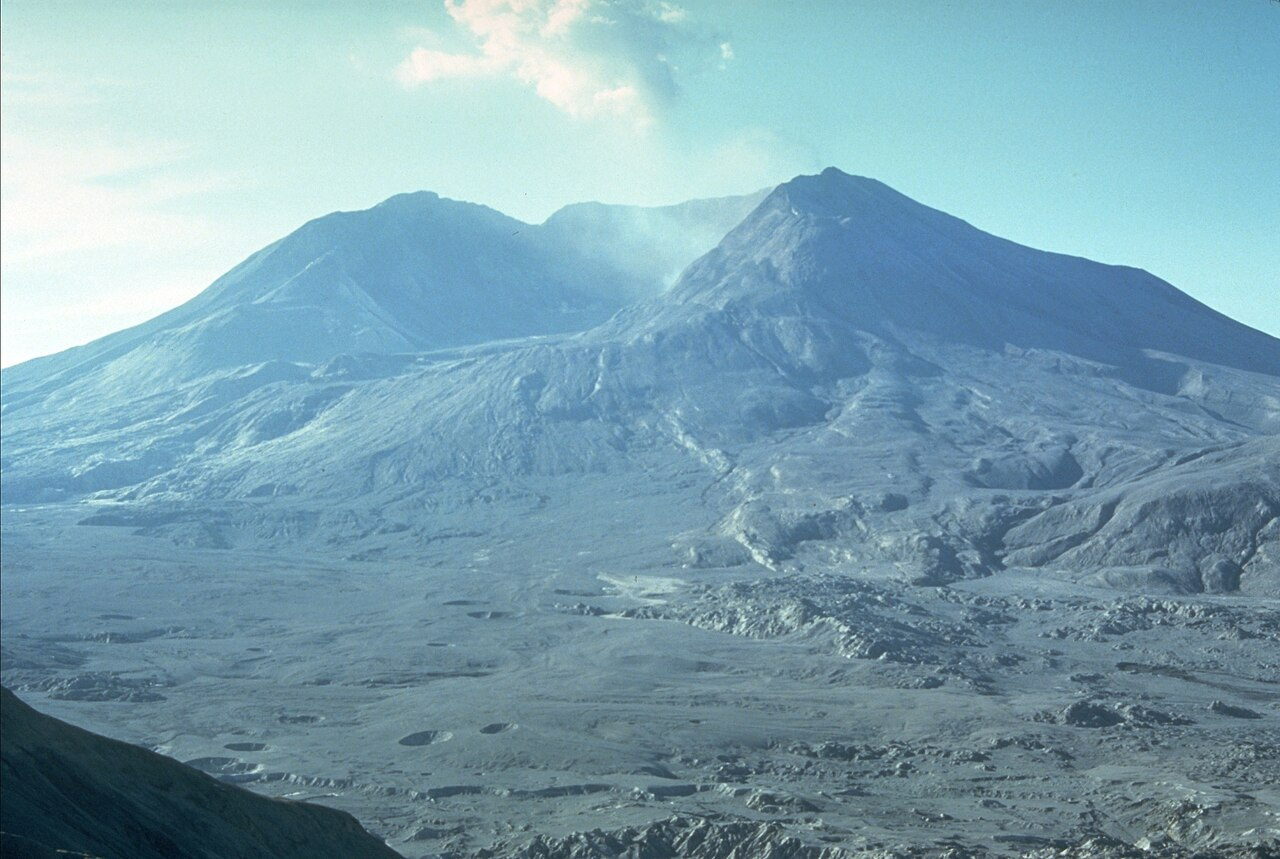
\includegraphics[width=\linewidth]{images/book1/g7-msh-after.jpg}

{\small 1980 年 9 月 10 日。}
\end{minipage}

{\small 从约翰斯顿山脊看到的圣海伦\omterm{def:g4:volcanoes-earthquakes-first-look:volcano}{火山}，\omterm{def:g4:volcanoes-earthquakes-first-look:eruption}{喷发}前后对比（1980 年 5 月 18 日）。
山顶和整个北侧已经消失，一个朝北开口的\omterm{def:g7:volcanoes:vent}{火山口}
取而代之。照片：Harry
Glicken，美国地质调查局（公有领域，经维基共享资源提供）。}
% ledger: commons:msh-before, commons:msh-after, usgs:msh-lead-up, usgs:msh-may18
\label{fig:g7:volcanoes:st-helens}
\end{omfigure}

本章我们将打开一座\omterm{def:g4:volcanoes-earthquakes-first-look:volcano}{火山}，看看是什么驱动了\omterm{def:g4:volcanoes-earthquakes-first-look:eruption}{喷发}；
我们将弄清为什么有些\omterm{def:g4:volcanoes-earthquakes-first-look:volcano}{火山}喷出平缓的\omterm{def:g4:volcanoes-earthquakes-first-look:eruption}{熔岩}\omterm{def:g1:landscapes-around-us:water}{河流}，而另一些\omterm{def:g4:volcanoes-earthquakes-first-look:volcano}{火山}
则把自身炸开；我们还将再看\omterm{def:g3:continents-and-oceans:world-map}{世界地图}，看看\omterm{def:g4:volcanoes-earthquakes-first-look:volcano}{火山}位于何处，
以及它们为何在那里。

\begin{recall}
\emph{\omterm{def:g4:volcanoes-earthquakes-first-look:volcano}{火山}}是地球内部深处的熔融\omterm{def:g3:stones-pebbles-sand:rock}{岩石}涌出地表的地方，
以及在那里堆积而成的小山或山峰。
\emph{\omterm{def:g4:volcanoes-earthquakes-first-look:eruption}{喷发}}时，\omterm{def:g4:volcanoes-earthquakes-first-look:volcano}{火山}喷出\omterm{def:g4:volcanoes-earthquakes-first-look:eruption}{熔岩}、\omterm{def:g4:volcanoes-earthquakes-first-look:eruption}{火山灰}和气体
（见\cref{ch:g4:volcanoes-earthquakes-first-look}）。\omterm{def:g6:inside-the-earth:layers}{地壳}之下，\omterm{def:g6:inside-the-earth:layers}{地幔}由炽热的
固态\omterm{def:g3:stones-pebbles-sand:rock}{岩石}构成，尽管它可以极其缓慢地蠕动
（见\cref{ch:g6:inside-the-earth}）。玄武岩和花岗岩都是\omterm{def:g6:rocks-and-minerals:rock-families}{火成岩}：
它们在熔融\omterm{def:g3:stones-pebbles-sand:rock}{岩石}冷却凝固时形成
（见\cref{ch:g6:rocks-and-minerals}）。地球的外层外壳被分割成若干板块，
这些板块每年移动几厘米；板块的边缘称为
\omterm{def:g7:plate-tectonics:plate-boundary}{板块边界}（见\cref{ch:g7:plate-tectonics}）。
\end{recall}

\section{火山内部}

\omterm{def:g6:inside-the-earth:layers}{地幔}是固态的。然而，在地表之下很深的一些地方，少量\omterm{def:g3:stones-pebbles-sand:rock}{岩石}会熔化。
熔融\omterm{def:g3:stones-pebbles-sand:rock}{岩石}比周围的固态\omterm{def:g3:stones-pebbles-sand:rock}{岩石}轻，
因此它会沿着裂隙缓慢上升，就像一滴
油在水中上浮一样。
% ledger: usgs:hawaii-hotspot (magma lighter than the surrounding rock, rises)

\begin{definition}[岩浆]\label{def:g7:volcanoes:magma}
\emph{岩浆}\index{岩浆}是地下的熔融\omterm{def:g3:stones-pebbles-sand:rock}{岩石}。它是一种炽热的液体，
其中可能含有晶体，并溶解有水蒸气、
二氧化碳等气体。喷出地表的岩浆称为
\omterm{def:g4:volcanoes-earthquakes-first-look:eruption}{熔岩}；它喷出时会失去大部分气体。
\end{definition}

上升的\omterm{def:g7:volcanoes:magma}{岩浆}常常在途中停止，停留在地表以下几千米处，
聚集成一个大的囊状体。在那里，它有时会等待数个世纪，
直到一次\omterm{def:g4:volcanoes-earthquakes-first-look:eruption}{喷发}将其中一部分排空。

\begin{definition}[岩浆房]\label{def:g7:volcanoes:magma-chamber}
\emph{岩浆房}\index{岩浆房}是\omterm{def:g4:volcanoes-earthquakes-first-look:volcano}{火山}下方\omterm{def:g3:stones-pebbles-sand:rock}{岩石}中的一个大空间，
位于\omterm{def:g4:volcanoes-earthquakes-first-look:volcano}{火山}之下几千米深处，\omterm{def:g7:volcanoes:magma}{岩浆}
在\omterm{def:g4:volcanoes-earthquakes-first-look:eruption}{喷发}前聚集于此。
\end{definition}

\begin{definition}[火山口通道与火山口]\label{def:g7:volcanoes:vent}
\emph{火山口通道}\index{火山口通道}是地表的一个开口，\omterm{def:g7:volcanoes:magma}{岩浆}、
气体和\omterm{def:g4:volcanoes-earthquakes-first-look:eruption}{火山灰}经由此喷出。\emph{火山口}\index{火山口}是
围绕\omterm{def:g4:volcanoes-earthquakes-first-look:volcano}{火山}口通道的碗状洼地，通常位于\omterm{def:g4:volcanoes-earthquakes-first-look:volcano}{火山}顶部。
\end{definition}

\begin{omfigure}
\begin{tikzpicture}[font=\small, x=1cm, y=1cm]
  % rocks below the volcano
  \fill[brown!25] (-6,-4.2) rectangle (6,0);
  \draw[brown!50] (-6,-1.4) -- (6,-1.4) (-6,-2.8) -- (6,-2.8);
  % the cone, built of layers of lava (dark) and ash (light)
  \fill[black!45] (-5.2,0) -- (-0.75,3.4) -- (0.75,3.4) -- (5.2,0) -- cycle;
    % layers dipping outwards, parallel to the flanks (slope 3.4/4.45)
  \foreach \k/\c in {0/black!25, 2/black!25, 4/black!25} {
    \pgfmathsetmacro{\xa}{-5.2+0.8*\k}\pgfmathsetmacro{\xb}{-5.2+0.8*(\k+1)}
    \pgfmathsetmacro{\ya}{(-0.18-\xa)*3.4/4.45}\pgfmathsetmacro{\yb}{(-0.18-\xb)*3.4/4.45}
    \fill[\c] (\xa,0) -- (-0.18,\ya) -- (-0.18,\yb) -- (\xb,0) -- cycle;
    \fill[\c] (-\xa,0) -- (0.18,\ya) -- (0.18,\yb) -- (-\xb,0) -- cycle;
  }
  % the crater at the top
  \fill[white] (-0.75,3.4) -- (-0.3,2.95) -- (0.3,2.95) -- (0.75,3.4) -- cycle;
  \draw[black!70] (-0.75,3.4) -- (-0.3,2.95) -- (0.3,2.95) -- (0.75,3.4);
  % magma chamber and the pipe up to the vent
  \fill[orange!85!red] (0,-3.0) ellipse (2.1 and 0.75);
  \fill[orange!85!red] (-0.18,-2.4) rectangle (0.18,2.98);
  % a side branch to a small side vent
  \fill[orange!85!red] (0.1,0.6) -- (2.55,1.5) -- (2.62,1.33) -- (0.1,0.25) -- cycle;
  % lava flow down the right flank, from the side vent
  \fill[orange!95!red] (2.5,1.45) .. controls (3.2,1.0) and (3.7,0.5) .. (4.6,0.08)
    -- (4.0,0.05) .. controls (3.3,0.4) and (2.9,0.8) .. (2.45,1.25) -- cycle;
  % ash column and gas
    \fill[black!22] (-0.3,3.0) -- (0.3,3.0) -- (0.45,3.9) -- (-0.45,3.9) -- cycle;
  \foreach \x/\y/\r in {0/3.95/0.45, -0.45/4.55/0.55, 0.45/4.6/0.5, -0.15/5.2/0.6,
                        0.6/5.3/0.5, -0.8/5.15/0.45, 0.15/5.8/0.55}
    \fill[black!22] (\x,\y) circle (\r);
  % labels
  \node[anchor=west] at (2.1,5.3) {火山灰和气体柱};
  \draw[black!60] (2.05,5.3) -- (1.05,5.2);
  \node[anchor=west] at (2.0,3.3) {火山口};
  \draw[black!60] (1.95,3.3) -- (0.6,3.2);
  \node[anchor=east] at (-2.0,3.8) {主火山口通道};
  \draw[black!60] (-1.95,3.75) -- (-0.1,3.0);
  \node[anchor=west] at (4.2,1.6) {侧火山口通道};
  \draw[black!60] (4.15,1.6) -- (2.65,1.45);
  \node[anchor=west] at (4.5,0.55) {熔岩流};
  \draw[black!60] (4.45,0.55) -- (3.9,0.4);
  \node[anchor=east, align=right] at (-3.0,1.75) {熔岩层与 \\火山灰层};
  \draw[black!60] (-2.95,1.6) -- (-2.2,1.1);
  \node[anchor=west, align=left] at (0.55,-0.9) {岩浆沿管道 \\上升};
  \draw[black!60] (0.5,-0.9) -- (0.2,-0.9);
  \node[anchor=west] at (2.3,-3.0) {岩浆房};
  \draw[black!60] (2.25,-3.0) -- (1.7,-3.0);
  \node[anchor=west, align=left, font=\footnotesize] at (-5.9,-3.7) {地下几千米};
  \draw[black!60, <->] (-4.3,0) -- (-4.3,-3.0);
\end{tikzpicture}

{\small \omterm{def:g4:volcanoes-earthquakes-first-look:volcano}{火山}剖面图（示意图，未按比例绘制）。\omterm{def:g7:volcanoes:magma}{岩浆}在
\omterm{def:g7:volcanoes:magma-chamber}{岩浆房}中汇聚，沿管道上升至位于\omterm{def:g7:volcanoes:vent}{火山口}底部的主\omterm{def:g7:volcanoes:vent}{火山口}；
一条分支通向山坡上的侧\omterm{def:g7:volcanoes:vent}{火山口}。每次\omterm{def:g4:volcanoes-earthquakes-first-look:eruption}{喷发}都会
为\omterm{def:g4:volcanoes-earthquakes-first-look:volcano}{火山}锥增加一层\omterm{def:g4:volcanoes-earthquakes-first-look:eruption}{熔岩}或\omterm{def:g4:volcanoes-earthquakes-first-look:eruption}{火山灰}。}
\label{fig:g7:volcanoes:cutaway}
\end{omfigure}

同一种熔融\omterm{def:g3:stones-pebbles-sand:rock}{岩石}有两个名称。在地下时它叫\emph{\omterm{def:g7:volcanoes:magma}{岩浆}}；一旦
从\omterm{def:g7:volcanoes:vent}{火山口}喷出，它就叫\emph{\omterm{def:g4:volcanoes-earthquakes-first-look:eruption}{熔岩}}。二者的区别不仅在于
措辞：\omterm{def:g7:volcanoes:magma}{岩浆}仍保有其中的气体，而\omterm{def:g4:volcanoes-earthquakes-first-look:eruption}{熔岩}已将大部分气体
逸散到空气中。我们将看到，这种气体决定了
\omterm{def:g4:volcanoes-earthquakes-first-look:volcano}{火山}的\omterm{def:g4:volcanoes-earthquakes-first-look:eruption}{喷发}类型。

\omterm{def:g7:volcanoes:magma}{岩浆}有多热？夏威夷\omterm{def:g4:volcanoes-earthquakes-first-look:volcano}{火山}观测站的科学家测得，
夏威夷\omterm{def:g4:volcanoes-earthquakes-first-look:volcano}{火山}之一基拉韦厄\omterm{def:g4:volcanoes-earthquakes-first-look:volcano}{火山}喷口流出的\omterm{def:g4:volcanoes-earthquakes-first-look:eruption}{熔岩}
温度约为\qty{1170}{\degreeCelsius}。炽热的\omterm{def:g3:stones-pebbles-sand:rock}{岩石}会发光，其颜色
取决于温度：专用照相机可以在远处读取\omterm{def:g4:volcanoes-earthquakes-first-look:eruption}{熔岩}流的温度，
方法是测量其发光的颜色。肉眼也能
大致判断温度，如下表所示。
% ledger: usgs:kilauea-temp, usgs:pyrometer

\begin{center}
\small
\begin{tabular}{|l|c|}
\hline
\textbf{发光\omterm{def:g3:stones-pebbles-sand:rock}{岩石}的颜色} & \textbf{温度} \\
\hline
黄色 & 约 1000 至 \qty{1200}{\degreeCelsius} \\
橙色 & 约 800 至 \qty{1000}{\degreeCelsius} \\
红色 & 约 600 至 \qty{800}{\degreeCelsius} \\
\hline
\end{tabular}
\end{center}
% ledger: usgs:kilauea-temp

\begin{remark}[一秒内冷却的表皮]\label{rem:g7:volcanoes:skin}
% ledger: usgs:kilauea-temp
\omterm{def:g4:volcanoes-earthquakes-first-look:eruption}{熔岩}刚接触空气时，表面每秒钟
降温数百度，炽热的\omterm{def:g3:stones-pebbles-sand:rock}{岩石}表面立即形成一层暗色的表皮。表皮之下
\omterm{def:g4:volcanoes-earthquakes-first-look:eruption}{熔岩}长时间保持高温。在夏威夷，\omterm{def:g4:volcanoes-earthquakes-first-look:eruption}{熔岩}曾在自身凝固的
顶盖下的\omterm{def:g4:volcanoes-earthquakes-first-look:eruption}{熔岩}隧道中流淌了\qty{10}{km}，从喷口一直流到
大海，到达岸边时温度仍约为\qty{1140}{\degreeCelsius}，
仅比喷口处低约 30 度。
\end{remark}

\begin{omfigure}
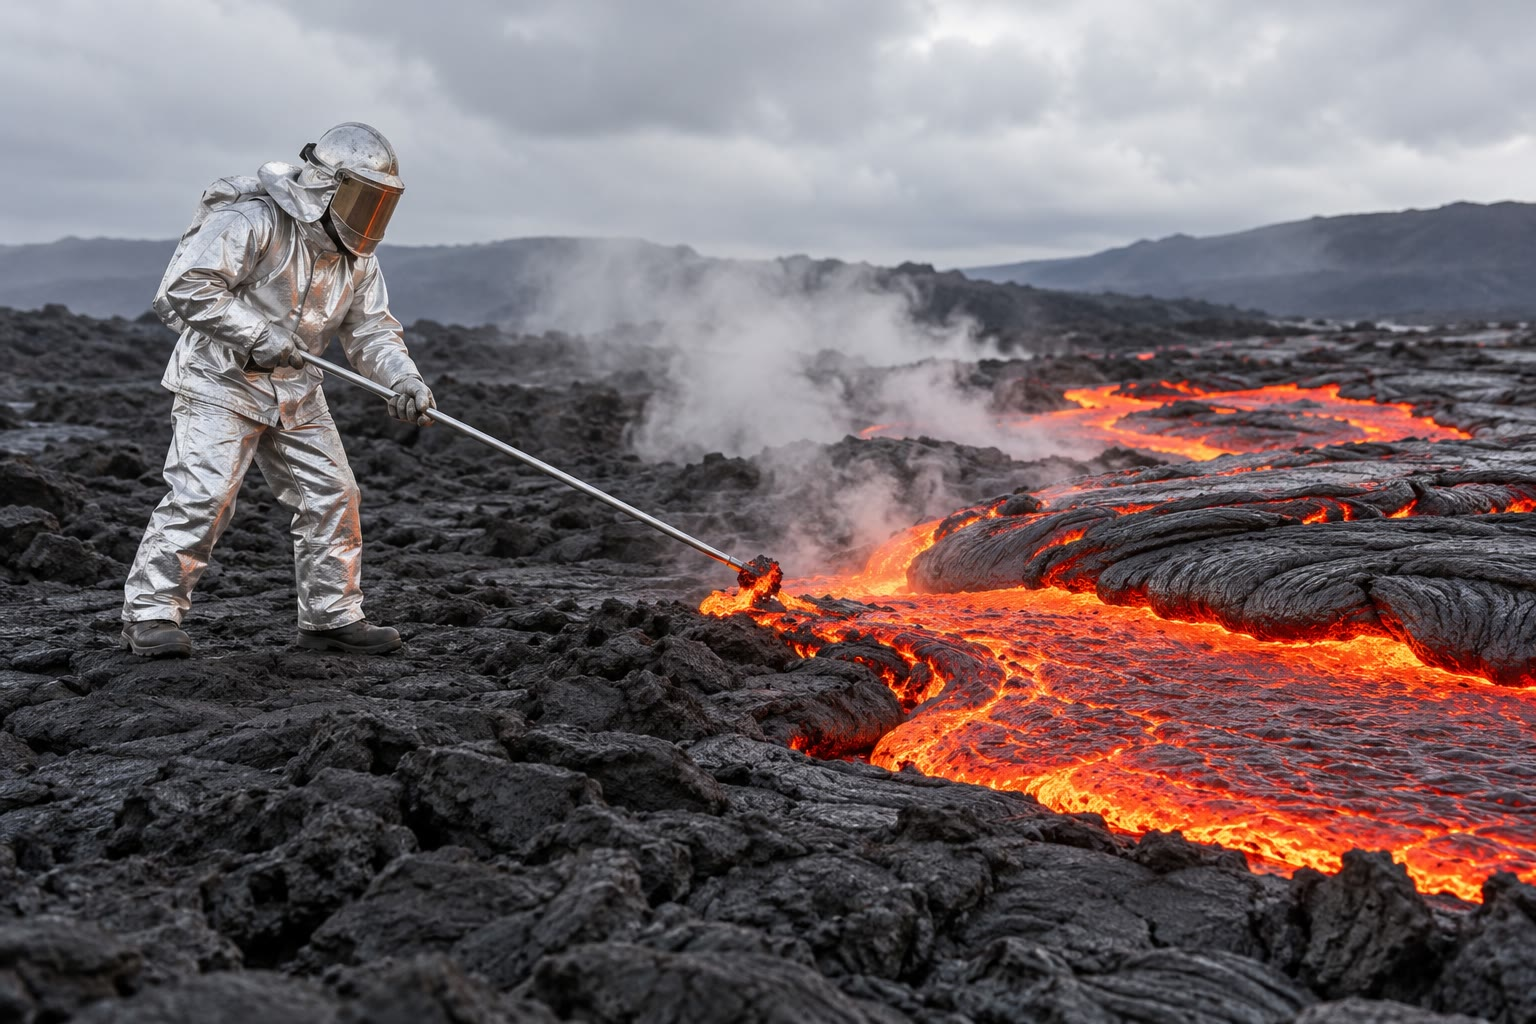
\includegraphics[width=0.6\linewidth]{images/book1/ai/g7-volcanologist.jpg}

{\small 一名身穿隔热反光服的\omterm{def:g4:volcanoes-earthquakes-first-look:volcano}{火山}学家，用长钢杆
取\omterm{def:g4:volcanoes-earthquakes-first-look:eruption}{熔岩}样本（AI 生成的通用场景示意图）。
只有受过专业训练、配备此类装备的科学家才会靠近流动的
\omterm{def:g4:volcanoes-earthquakes-first-look:eruption}{熔岩}；其他人只能在有关部门允许的地方观看。}
\label{fig:g7:volcanoes:volcanologist}
\end{omfigure}

\section{两种喷发方式}

圣海伦斯山曾自行炸裂。与之相反，夏威夷的\omterm{def:g4:volcanoes-earthquakes-first-look:volcano}{火山}
通常喷出\omterm{def:g4:volcanoes-earthquakes-first-look:eruption}{熔岩}，\omterm{def:g4:volcanoes-earthquakes-first-look:eruption}{熔岩}沿山坡向下流走。
地质学家将\omterm{def:g4:volcanoes-earthquakes-first-look:eruption}{喷发}分为两类。

\begin{definition}[溢流式喷发与爆炸式喷发]\label{def:g7:volcanoes:eruption-types}
在\emph{溢流式喷发}\index{溢流式喷发}中，\omterm{def:g7:volcanoes:magma}{岩浆}
平静地以\omterm{def:g4:volcanoes-earthquakes-first-look:eruption}{熔岩}形式涌出，\omterm{def:g4:volcanoes-earthquakes-first-look:eruption}{熔岩}从\omterm{def:g7:volcanoes:vent}{火山口}流走，有时可流动数千米，
或以炽热熔滴的喷泉形式喷出。在\emph{爆炸式
喷发}\index{爆炸式喷发}中，\omterm{def:g7:volcanoes:magma}{岩浆}被自身的气体炸成碎片，
\omterm{def:g4:volcanoes-earthquakes-first-look:eruption}{火山灰}、气体和岩块组成的柱体被抛入
高空。
\end{definition}

\begin{omfigure}
\begin{minipage}[t]{0.49\linewidth}\centering
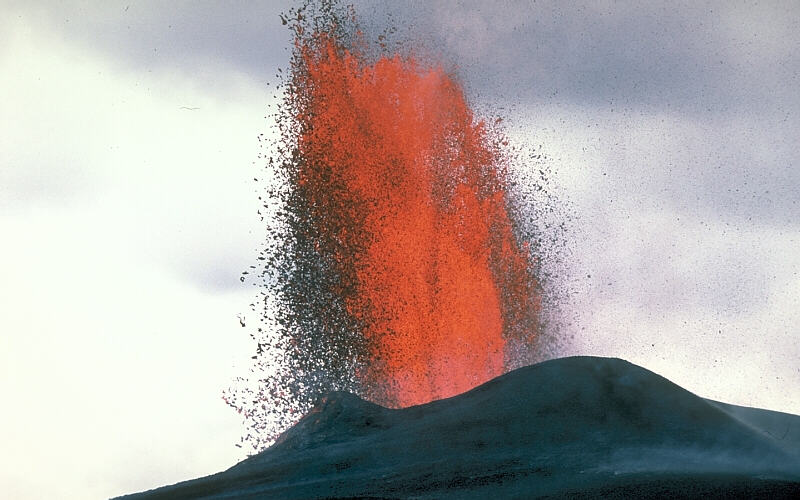
\includegraphics[height=4.5cm]{images/book1/g7-lava-fountain.jpg}

{\small 溢流式：1983 年夏威夷基拉韦厄\omterm{def:g4:volcanoes-earthquakes-first-look:volcano}{火山}的\omterm{def:g4:volcanoes-earthquakes-first-look:eruption}{熔岩}喷泉。
照片：J.~D. Griggs, USGS.}
\end{minipage}\hfill
\begin{minipage}[t]{0.49\linewidth}\centering
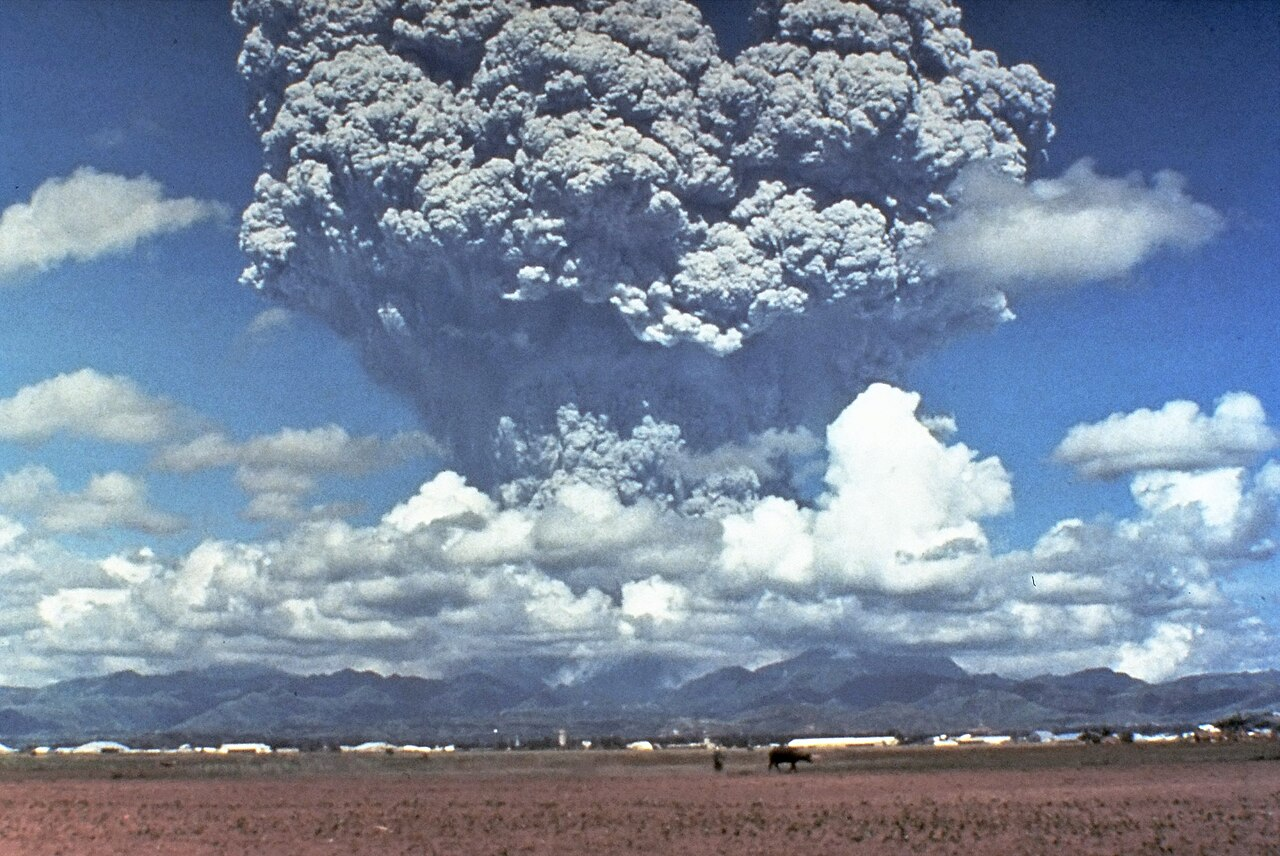
\includegraphics[height=4.5cm]{images/book1/g7-pinatubo.jpg}

{\small 爆炸式：菲律宾皮纳图博\omterm{def:g4:volcanoes-earthquakes-first-look:volcano}{火山}的\omterm{def:g4:volcanoes-earthquakes-first-look:eruption}{喷发}柱，
1991 年 6 月 12 日。照片：Dave Harlow, USGS.}
\end{minipage}\par\medskip


{\small 两张照片均属公有领域（经由
维基共享资源）。}
% ledger: commons:lava-fountain, commons:pinatubo
\label{fig:g7:volcanoes:two-photos}
\end{omfigure}

是什么造成了这种差异？主要有两个因素：\omterm{def:g7:volcanoes:magma}{岩浆}的流动性，
以及其所含气体的多少。

\textbf{流动或黏稠。}有些\omterm{def:g7:volcanoes:magma}{岩浆}流动性强，接近温热的蜂蜜：这种
\omterm{def:g7:volcanoes:magma}{岩浆}冷却后形成深色的玄武岩，夏威夷即是这种情况。另一些
\omterm{def:g7:volcanoes:magma}{岩浆}浓稠而黏，像冷蜂蜜或牙膏。在流动性强的
\omterm{def:g7:volcanoes:magma}{岩浆}中，气泡容易上升，并在表面逸出，每次只有少量。
在黏性\omterm{def:g7:volcanoes:magma}{岩浆}中，气泡则被困住。

\textbf{气体少还是多。}一瓶汽水中溶有大量气体，
这些气体溶解在水中，由密封瓶内的压强维持其溶解状态，
肉眼看不见。打开瓶盖，压强降低，气泡
随处出现；若瓶子曾被摇晃，泡沫便会冲出。
地下深处的\omterm{def:g7:volcanoes:magma}{岩浆}同样在高压下溶有气体。\omterm{def:g7:volcanoes:magma}{岩浆}上升时，
压强降低，气体便从溶液中析出，形成气泡。
% ledger: usgs:volcanic-gases

综合两者来看：气体少而流动性强的\omterm{def:g7:volcanoes:magma}{岩浆}，气泡会逸出，
并以流动的\omterm{def:g4:volcanoes-earthquakes-first-look:eruption}{熔岩}形式喷出，\omterm{def:g4:volcanoes-earthquakes-first-look:eruption}{喷发}属于溢流式。满含气体的黏性\omterm{def:g7:volcanoes:magma}{岩浆}
会保留其中的气泡，直至气泡膨胀到足以将\omterm{def:g7:volcanoes:magma}{岩浆}撕裂
成碎片，\omterm{def:g4:volcanoes-earthquakes-first-look:eruption}{喷发}属于爆炸式。泡沫状\omterm{def:g7:volcanoes:magma}{岩浆}的碎片
在空中凝固成\omterm{def:g4:volcanoes-earthquakes-first-look:eruption}{火山灰}和浮岩，浮岩中气泡极多，
以至能够漂浮。

\begin{example}[皮纳图博火山，1991 年：走了气的汽水与摇过的汽水]\label{ex:g7:volcanoes:pinatubo}
% ledger: usgs:pinatubo-1991
1991 年 6 月，首批\omterm{def:g7:volcanoes:magma}{岩浆}抵达菲律宾皮纳图博\omterm{def:g4:volcanoes-earthquakes-first-look:volcano}{火山}的
地表。\omterm{def:g7:volcanoes:magma}{岩浆}在上升途中已失去大部分气体，“像一瓶
走了气的汽水”，这是当时观测者的原话。
\omterm{def:g7:volcanoes:magma}{岩浆}缓慢溢出，在\omterm{def:g7:volcanoes:vent}{火山口}上方堆成一座小丘，没有爆炸。
随后，6 月 12 日，仍富含气体的\omterm{def:g7:volcanoes:magma}{岩浆}抵达地表并爆发，
即上图中的\omterm{def:g4:volcanoes-earthquakes-first-look:eruption}{喷发}柱。6 月 15 日，气体更为丰富的\omterm{def:g7:volcanoes:magma}{岩浆}到达，
\omterm{def:g4:volcanoes-earthquakes-first-look:volcano}{火山}发生了 20 世纪最大规模的\omterm{def:g4:volcanoes-earthquakes-first-look:eruption}{喷发}之一：
喷出 5 立方千米以上的\omterm{def:g3:stones-pebbles-sand:rock}{岩石}和\omterm{def:g4:volcanoes-earthquakes-first-look:eruption}{火山灰}，\omterm{def:g4:volcanoes-earthquakes-first-look:eruption}{火山灰}云升至
\qty{35}{km} 高，山顶塌陷成一个直径为 \qty{2.5}{km} 的
洼坑。同一座\omterm{def:g4:volcanoes-earthquakes-first-look:volcano}{火山}，同一周
——气体造成了差别。
\end{example}

\omterm{def:g4:volcanoes-earthquakes-first-look:volcano}{火山}的形状保留着它历次\omterm{def:g4:volcanoes-earthquakes-first-look:eruption}{喷发}的痕迹。流动性强的\omterm{def:g4:volcanoes-earthquakes-first-look:eruption}{熔岩}
流得很远才凝固，因此一层层堆积成宽阔的山体，
坡度平缓，形如平放于地面的武士盾牌，属于
\emph{盾状\omterm{def:g4:volcanoes-earthquakes-first-look:volcano}{火山}}。夏威夷的莫纳罗亚\omterm{def:g4:volcanoes-earthquakes-first-look:volcano}{火山}便是一例。黏稠的\omterm{def:g4:volcanoes-earthquakes-first-look:eruption}{熔岩}与\omterm{def:g4:volcanoes-earthquakes-first-look:eruption}{火山灰}
堆积在靠近火口处，形成陡峭的锥体，由\omterm{def:g4:volcanoes-earthquakes-first-look:eruption}{熔岩}与\omterm{def:g4:volcanoes-earthquakes-first-look:eruption}{火山灰}的层层叠加构成：
\emph{层状\omterm{def:g4:volcanoes-earthquakes-first-look:volcano}{火山}}（\emph{strata}意为层）。圣海伦斯\omterm{def:g4:volcanoes-earthquakes-first-look:volcano}{火山}
与皮纳图博\omterm{def:g4:volcanoes-earthquakes-first-look:volcano}{火山}都属此类。

\begin{omfigure}
\begin{tikzpicture}[font=\small, x=1cm, y=1cm]
  % --- left: effusive, a shield
  \begin{scope}
    \fill[brown!25] (-3.3,-1.2) rectangle (3.3,0);
    \fill[black!50] (-3.3,0) .. controls (-2.0,0.45) and (-1.0,1.0) .. (-0.35,1.25)
      -- (0.35,1.25) .. controls (1.0,1.0) and (2.0,0.45) .. (3.3,0) -- cycle;
    \fill[orange!85!red] (-0.12,-1.2) rectangle (0.12,1.25);
    % fountain
    \foreach \a in {-25,-12,0,12,25}
      \draw[orange!90!red, line width=0.9pt] (0,1.25) .. controls ({0.4*sin(\a)},2.2) .. ({1.0*sin(\a)},1.6);
    % lava flows far down the gentle slopes
    \draw[orange!95!red, line width=2.2pt, line cap=round] (0.3,1.22) .. controls (1.2,0.95) and (2.1,0.45) .. (3.1,0.08);
    \draw[orange!95!red, line width=2.2pt, line cap=round] (-0.3,1.22) .. controls (-1.3,0.95) and (-2.2,0.45) .. (-3.0,0.1);
    \node[font=\small\bfseries] at (0,4.3) {溢流式};
    \node[align=center, font=\footnotesize] at (0,-1.75) {岩浆流动性强，气体少：\\熔岩流得远；宽盾形};
    \node[anchor=west, font=\footnotesize] at (1.2,1.9) {熔岩喷泉};
    \draw[black!60] (1.15,1.9) -- (0.6,1.75);
    \node[anchor=west, font=\footnotesize, align=left] at (1.9,1.2) {熔岩长距离 \\流动};
    \draw[black!60] (1.85,1.05) -- (1.5,0.82);
  \end{scope}
  % --- right: explosive, a steep cone
  \begin{scope}[xshift=7.4cm]
    \fill[brown!25] (-3.3,-1.2) rectangle (3.3,0);
    \fill[black!45] (-2.3,0) -- (-0.4,2.2) -- (0.4,2.2) -- (2.3,0) -- cycle;
    \fill[orange!85!red] (-0.12,-1.2) rectangle (0.12,2.2);
    \foreach \x/\y/\r in {0/2.6/0.35, -0.3/3.05/0.4, 0.3/3.1/0.38, 0/3.5/0.45, -0.45/3.55/0.32, 0.45/3.6/0.32}
      \fill[black!28] (\x,\y) circle (\r);
    % pyroclastic flow down the flank
    \fill[black!30] (0.45,2.1) .. controls (1.0,1.5) and (1.6,0.7) .. (2.9,0.05)
      -- (2.2,0.05) .. controls (1.4,0.45) and (0.9,1.2) .. (0.35,1.95) -- cycle;
    \node[font=\small\bfseries] at (0,4.3) {爆炸式};
    \node[align=center, font=\footnotesize] at (0,-1.75) {黏性岩浆，气体多：\\火山灰柱；陡峭锥体};
    \node[anchor=west, font=\footnotesize] at (0.9,3.4) {火山灰柱};
    \draw[black!60] (0.85,3.4) -- (0.7,3.4);
    \node[anchor=west, font=\footnotesize, align=left] at (1.8,1.35) {火山碎屑 \\流};
    \draw[black!60] (1.75,1.35) -- (1.3,1.0);
  \end{scope}
\end{tikzpicture}

{\small 两种\omterm{def:g4:volcanoes-earthquakes-first-look:eruption}{喷发}类型及其所形成的\omterm{def:g4:volcanoes-earthquakes-first-look:volcano}{火山}（示意图，
非按比例）。}
\label{fig:g7:volcanoes:two-kinds}
\end{omfigure}

\begin{method}[溢流式还是爆炸式？四条线索]\label{met:g7:volcanoes:clues}
要根据文字描述或照片判断一座\omterm{def:g4:volcanoes-earthquakes-first-look:volcano}{火山}属于哪种\omterm{def:g4:volcanoes-earthquakes-first-look:eruption}{喷发}，
可以寻找以下线索。
\begin{enumerate}
  \item \emph{喷出的是什么？}\omterm{def:g4:volcanoes-earthquakes-first-look:eruption}{熔岩}流动或呈喷泉状喷涌：
        属于溢流式。\omterm{def:g4:volcanoes-earthquakes-first-look:eruption}{火山灰}柱、抛出的岩块：属于爆炸式。
  \item \emph{\omterm{def:g4:volcanoes-earthquakes-first-look:volcano}{火山}的形状。}宽阔的山体，坡度平缓：
        多为\omterm{def:g7:volcanoes:eruption-types}{溢流式喷发}。陡峭的锥体：多为爆炸式。
  \item \emph{\omterm{def:g7:volcanoes:magma}{岩浆}。}流动性强、气体少：溢流式。黏稠、气体多：
        爆炸式。
  \item \emph{遗留的\omterm{def:g3:stones-pebbles-sand:rock}{岩石}。}深色、坚硬的\omterm{def:g4:volcanoes-earthquakes-first-look:eruption}{熔岩}流：溢流式。
        \omterm{def:g4:volcanoes-earthquakes-first-look:eruption}{火山灰}与浮岩的层：爆炸式。
\end{enumerate}
\end{method}

\begin{example}[运用线索]\label{ex:g7:volcanoes:clues}
一位旅行者描述一座\omterm{def:g4:volcanoes-earthquakes-first-look:volcano}{火山}：“一座巨大、轮廓圆缓的山，
山坡上到处是黑色的\omterm{def:g4:volcanoes-earthquakes-first-look:eruption}{熔岩}流，其中有些只有几年历史。”
线索 2（坡面平缓）与线索 4（深色\omterm{def:g4:volcanoes-earthquakes-first-look:eruption}{熔岩}流）都指向\omterm{def:g7:volcanoes:eruption-types}{溢流式喷发}：
它是一座盾状\omterm{def:g4:volcanoes-earthquakes-first-look:volcano}{火山}，类似夏威夷的莫纳罗亚\omterm{def:g4:volcanoes-earthquakes-first-look:volcano}{火山}。
\end{example}

\begin{inthelab}[瓶中的火山（课堂上，在教师指导下）]
教师取来两瓶密封的气泡水，一瓶静置，
另一瓶被轻轻摇过。两瓶都在室外打开，
瓶口朝向远离众人的方向，对着水盆。静置的那瓶发出嘶嘶声，
只冒出几个气泡；摇过的那瓶则涌出泡沫，喷射而出。
哪一瓶像夏威夷的\omterm{def:g7:volcanoes:magma}{岩浆}，哪一瓶像皮纳图博的\omterm{def:g7:volcanoes:magma}{岩浆}？接着，
把一块浮岩和一颗\omterm{def:g3:stones-pebbles-sand:pebble}{卵石}放入一碗水中：浮岩漂浮。
用放大镜观察，浮岩布满孔洞，
那是\omterm{def:g7:volcanoes:magma}{岩浆}\omterm{def:g4:volcanoes-earthquakes-first-look:eruption}{喷发}时被凝固在\omterm{def:g3:stones-pebbles-sand:rock}{岩石}中的气泡。
\end{inthelab}

\section{火山喷出的物质}

\omterm{def:g4:volcanoes-earthquakes-first-look:eruption}{喷发}喷出的远不止\omterm{def:g4:volcanoes-earthquakes-first-look:eruption}{熔岩}，还有气体、\omterm{def:g4:volcanoes-earthquakes-first-look:eruption}{火山灰}、
岩块，严重时甚至会出现炽热的\omterm{def:g4:volcanoes-earthquakes-first-look:eruption}{火山灰}崩。

含量最多的气体远超其他，是水蒸气。大规模\omterm{def:g4:volcanoes-earthquakes-first-look:eruption}{喷发}
会在短时间内释放出大量气体。仅在 1991 年的某一天，
皮纳图博\omterm{def:g4:volcanoes-earthquakes-first-look:volcano}{火山}被认为在那一天向高层大气中送出了
超过 2.5 亿吨气体。
% ledger: usgs:volcanic-gases

\begin{definition}[火山碎屑流]\label{def:g7:volcanoes:pyroclastic-flow}
称\emph{火山碎屑流}\index{火山碎屑流}为一种快速的崩落物流，
由炽热的气体、\omterm{def:g4:volcanoes-earthquakes-first-look:eruption}{火山灰}和岩块组成，岩块大小从尘粒到巨石不等，
在\omterm{def:g7:volcanoes:eruption-types}{爆炸式喷发}时沿\omterm{def:g4:volcanoes-earthquakes-first-look:volcano}{火山}斜坡急速冲下。
（\emph{Pyro} 意为火，\emph{clastic} 意为碎屑。）
\end{definition}

\omterm{def:g7:volcanoes:pyroclastic-flow}{火山碎屑流}通常以超过 \qty{80}{km/h} 的速度运动，其中的\omterm{def:g3:stones-pebbles-sand:rock}{岩石}
和气体的温度一般在 200 至 \qty{700}{\degreeCelsius} 之间。
它们一般沿\omterm{def:g1:landscapes-around-us:landform}{山谷}流动，像水一样，几乎摧毁、烧毁或掩埋
沿途的一切。1980 年 5 月 18 日，圣海伦斯\omterm{def:g4:volcanoes-earthquakes-first-look:volcano}{火山}的\omterm{def:g7:volcanoes:pyroclastic-flow}{火山碎屑流}
以 80 至 \qty{130}{km/h} 的速度疾驰，温度至少
为 \qty{700}{\degreeCelsius}，并蔓延至距\omterm{def:g7:volcanoes:vent}{火山口} \qty{8}{km} 处。
% ledger: usgs:pyroclastic-flows, usgs:msh-flows, usgs:msh-reach

下表概括了\omterm{def:g4:volcanoes-earthquakes-first-look:volcano}{火山}的各类产物。

\begin{center}
\small
\begin{tabular}{|p{0.2\linewidth}|p{0.4\linewidth}|p{0.3\linewidth}|}
\hline
\textbf{产物} & \textbf{性质} & \textbf{危害} \\
\hline
\omterm{def:g4:volcanoes-earthquakes-first-look:eruption}{熔岩}流 & 熔融\omterm{def:g3:stones-pebbles-sand:rock}{岩石}在地面流动，随后凝固 & 烧毁、掩埋途经之物，但通常流速较慢，人们可以及时避开 \\
\hline
\omterm{def:g4:volcanoes-earthquakes-first-look:eruption}{火山灰} & 喷入空中的细小\omterm{def:g3:stones-pebbles-sand:rock}{岩石}和玻璃碎屑 & 落至远处；屋顶会因其重量而坍塌；会损坏飞机 \\
\hline
\omterm{def:g4:volcanoes-earthquakes-first-look:volcano}{火山}弹 & 被抛出的\omterm{def:g4:volcanoes-earthquakes-first-look:eruption}{熔岩}块，飞行中逐渐凝固 & 在\omterm{def:g7:volcanoes:vent}{火山口通道}附近砸毁所击中之物 \\
\hline
气体 & 主要是水蒸气，其次是二氧化碳和二氧化硫 & 部分气体有毒；二氧化碳会在低洼处聚集 \\
\hline
\omterm{def:g7:volcanoes:pyroclastic-flow}{火山碎屑流} & 炽热的\omterm{def:g4:volcanoes-earthquakes-first-look:eruption}{火山灰}、\omterm{def:g3:stones-pebbles-sand:rock}{岩石}和气体形成的崩落物流 & 最致命：速度太快、温度太高，无法逃离 \\
\hline
泥流 & \omterm{def:g4:volcanoes-earthquakes-first-look:eruption}{火山灰}和\omterm{def:g3:stones-pebbles-sand:rock}{岩石}与雨水或融雪混合而成 & 沿\omterm{def:g1:landscapes-around-us:landform}{山谷}急速冲下，有时远离\omterm{def:g4:volcanoes-earthquakes-first-look:volcano}{火山} \\
\hline
\end{tabular}
\end{center}
% ledger: usgs:lava-flows, usgs:volcanic-gases, usgs:pyroclastic-flows, usgs:pinatubo-1991, usgs:msh-flows

\begin{method}[需要多长时间？]\label{met:g7:volcanoes:time}
要求以已知速度运动的物体走完一段距离所需的时间，
用距离除以速度：
\[
\text{时间} = \frac{\text{距离}}{\text{速度}}.
\]
若距离以千米、速度以千米每小时为单位，所得时间
以小时为单位；乘以 60 即可得分钟数。
\end{method}

\begin{example}[与火山碎屑流赛跑]\label{ex:g7:volcanoes:race}
一股以 \qty{120}{km/h} 的速度运动的\omterm{def:g7:volcanoes:pyroclastic-flow}{火山碎屑流}，正冲向
沿\omterm{def:g1:landscapes-around-us:landform}{山谷}下游 \qty{6}{km} 处的一个村庄。所需时间为 $6 \div 120 = 0.05$ 小时，即
$0.05 \times 60 = 3$ 分钟。仅有 3 分钟，无人能跑出，
甚至开车也来不及离开\omterm{def:g1:landscapes-around-us:landform}{山谷}。只有在\omterm{def:g4:volcanoes-earthquakes-first-look:volcano}{火山}\omterm{def:g4:volcanoes-earthquakes-first-look:eruption}{喷发}
\emph{之前}离开的人，才是安全的。
\end{example}

\begin{remark}[泥流：之后才到来的危险]\label{rem:g7:volcanoes:mudflows}
% ledger: usgs:msh-flows, usgs:pinatubo-lahars
\omterm{def:g4:volcanoes-earthquakes-first-look:eruption}{喷发}之后，斜坡上会覆盖着松散的\omterm{def:g4:volcanoes-earthquakes-first-look:eruption}{火山灰}。雨水落下时，
或者当高温融化山顶的积雪和冰层时，\omterm{def:g4:volcanoes-earthquakes-first-look:eruption}{火山灰}便会变成
沿\omterm{def:g1:landscapes-around-us:landform}{山谷}急速冲下的泥流。1980 年 5 月 18 日，圣海伦斯\omterm{def:g4:volcanoes-earthquakes-first-look:volcano}{火山}的
泥流损毁了 27 座桥梁和近 200 座房屋。在
皮纳图博\omterm{def:g4:volcanoes-earthquakes-first-look:volcano}{火山}周边，随后数年的暴雨将\omterm{def:g4:volcanoes-earthquakes-first-look:eruption}{火山灰}冲成
巨大的泥流，掩埋了整个村庄：其造成的破坏甚至超过
\omterm{def:g4:volcanoes-earthquakes-first-look:eruption}{喷发}本身。
\end{remark}


\section{火山分布在哪里？}

位于华盛顿的史密森学会保存着一份名录，
收录了过去 12\,000 年内已知曾经\omterm{def:g4:volcanoes-earthquakes-first-look:eruption}{喷发}的全部\omterm{def:g4:volcanoes-earthquakes-first-look:volcano}{火山}，共 1\,214 座，
既有陆上的，也有海底的。名录为每座\omterm{def:g4:volcanoes-earthquakes-first-look:volcano}{火山}注明
其与板块的位置关系。下图即按此方式着色。
% ledger: data:gvp (counts computed in figdata/grade-7/volcano_settings.py)

\begin{omfigure}
\begin{tikzpicture}
\begin{axis}[ommap, width=\linewidth, xtick={-180,-90,...,180}, ytick={-60,0,60},
  legend style={at={(0.02,0.04)}, anchor=south west, font=\scriptsize,
  fill=white, fill opacity=0.85, text opacity=1, draw=black!40}, legend cell align=left]
\addplot[fill=omLithAlluv, draw=black!45, line width=0.2pt, forget plot] table {figdata/out/shared-geo-land.dat};
\addplot[omRidge!60, line width=0.5pt, forget plot] table {figdata/out/shared-geo-school-ridge.dat};
\addplot[omTrench!60, line width=0.5pt, forget plot] table {figdata/out/shared-geo-school-subduction.dat};
\addplot[only marks, mark=triangle*, mark size=1.3pt, omTrench, forget plot] table {figdata/out/grade-7-volcano_settings-map-sub.dat};
\addplot[only marks, mark=triangle*, mark size=1.3pt, omRidge, forget plot] table {figdata/out/grade-7-volcano_settings-map-rift.dat};
\addplot[only marks, mark=*, mark size=1.4pt, orange!90!black, forget plot] table {figdata/out/grade-7-volcano_settings-map-intra.dat};
\addlegendimage{only marks, mark=triangle*, mark size=1.6pt, omTrench}
\addlegendentry{板块俯冲处}
\addlegendimage{only marks, mark=triangle*, mark size=1.6pt, omRidge}
\addlegendentry{板块分离处}
\addlegendimage{only marks, mark=*, mark size=1.6pt, orange!90!black}
\addlegendentry{板块内部}
\end{axis}
\end{tikzpicture}

{\small 过去 12\,000 年内活动的\omterm{def:g4:volcanoes-earthquakes-first-look:volcano}{火山}，按其所处的
位置着色。浅色线条为\omterm{def:g7:plate-tectonics:plate-boundary}{板块边界}，其中板块分离处
（红色）及板块俯冲处（蓝色）。数据来源：史密森学会
全球\omterm{def:g4:volcanoes-earthquakes-first-look:volcano}{火山}活动计划；\omterm{def:g7:plate-tectonics:plate-boundary}{板块边界}据 P.~Bird（2003）；\omterm{def:g1:landscapes-around-us:water}{海岸}线取自
Natural Earth。}
% ledger: data:gvp, data:pb2002, data:ne-land
\label{fig:g7:volcanoes:map}
\end{omfigure}

\begin{omfigure}
\begin{tikzpicture}
  \begin{axis}[xbar, width=0.72\linewidth, height=3.6cm, bar width=8pt,
      xmin=0, xmax=1000, ymin=-0.6, ymax=3.6, y dir=reverse,
      ytick={0,...,3}, yticklabels={{一个板块俯冲到另一个之下处},{板块相互分离处},{板块内部},{未知}},
      xlabel={火山数量},
      axis x line=bottom, axis y line=left, axis line style={-},
      tick label style={font=\scriptsize}, label style={font=\small},
      nodes near coords, nodes near coords style={font=\scriptsize, anchor=west},
      point meta=explicit symbolic, enlarge y limits=false, clip=false]
    \addplot[fill=black!30, draw=black!60] table[x=n, y=idx, meta=n] {figdata/out/grade-7-volcano_settings.dat};
  \end{axis}
\end{tikzpicture}

{\small 在 1\,214 座\omterm{def:g4:volcanoes-earthquakes-first-look:volcano}{火山}中，各有多少座位于每种构造环境。}
% ledger: data:gvp (figdata/grade-7/volcano_settings.py, main table)
\label{fig:g7:volcanoes:counts}
\end{omfigure}

\begin{proposition}[大多数火山位于板块边界]\label{prop:g7:volcanoes:where}
% ledger: data:gvp (counts computed in figdata/grade-7/volcano_settings.py)
过去 12\,000 年内活动的 1\,214 座\omterm{def:g4:volcanoes-earthquakes-first-look:volcano}{火山}中，838 座（69~\%）位于一块板块俯冲到另一块板块之下的地方，
221 座（18~\%）位于板块相互远离的地方；
149 座（12~\%）位于板块内部，远离其边缘。对于
最后 6 座（0.5~\%），其所处的构造环境未知。
\end{proposition}

\textbf{板块相互远离的地方。}沿洋脊，以及东非正在被撕裂的那类裂谷，
板块彼此拉开。
\omterm{def:g7:volcanoes:magma}{岩浆}从\omterm{def:g6:inside-the-earth:layers}{地幔}上升，进入不断加宽的裂缝并将其充填，
于是形成新的\omterm{def:g6:inside-the-earth:layers}{地壳}。大多数洋脊位于海底，但冰岛正好坐落在大西洋中脊上：
在这里，这些\omterm{def:g4:volcanoes-earthquakes-first-look:volcano}{火山}可以在陆地上看到。
它们的\omterm{def:g7:volcanoes:magma}{岩浆}大多是流动性强的玄武岩，\omterm{def:g4:volcanoes-earthquakes-first-look:eruption}{喷发}多为
溢流式。
% ledger: usgs:arc-magma, usgs:iceland, usgs:east-africa

\textbf{一块板块俯冲到另一块板块之下的地方。}超过三分之二的\omterm{def:g4:volcanoes-earthquakes-first-look:volcano}{火山}位于此类地方，
沿太平洋边缘排列成线，
即——“火环”——以及少数其他地方。在深处，沿着
俯冲的板块，部分\omterm{def:g3:stones-pebbles-sand:rock}{岩石}发生熔融；科学家至今仍在讨论
究竟是哪一种\omterm{def:g3:stones-pebbles-sand:rock}{岩石}熔融，是俯冲的板块、上覆的板块，还是两者都有。
此处上升的\omterm{def:g7:volcanoes:magma}{岩浆}通常黏稠且富含气体：这些就是
爆炸式\omterm{def:g4:volcanoes-earthquakes-first-look:volcano}{火山}，例如圣海伦斯\omterm{def:g4:volcanoes-earthquakes-first-look:volcano}{火山}和皮纳图博\omterm{def:g4:volcanoes-earthquakes-first-look:volcano}{火山}。数据证实了这一点：
在列表中的 660 座陡峭的锥状\omterm{def:g4:volcanoes-earthquakes-first-look:volcano}{火山}（层状\omterm{def:g4:volcanoes-earthquakes-first-look:volcano}{火山}）中，564 座——即 85~\%——
位于一块板块俯冲到另一块板块之下的地方。
% ledger: usgs:arc-magma, data:gvp (figdata/grade-7/volcano_settings.py, part strato)

\textbf{板块内部。}少数\omterm{def:g4:volcanoes-earthquakes-first-look:volcano}{火山}远离任何边界。
其中最著名的是夏威夷的\omterm{def:g4:volcanoes-earthquakes-first-look:volcano}{火山}，它们位于太平洋中部，
距离板块最近的边缘超过 \qty{3200}{km}。
% ledger: usgs:hawaii-hotspot

\begin{definition}[热点]\label{def:g7:volcanoes:hotspot}
\emph{热点}\index{热点}是\omterm{def:g6:inside-the-earth:layers}{地幔}深处的一个地点，它
能持续数百万年保持高温，并不断向
地表的\omterm{def:g4:volcanoes-earthquakes-first-look:volcano}{火山}输送\omterm{def:g7:volcanoes:magma}{岩浆}，即使远离板块边缘也是如此。
\end{definition}

\omterm{def:g7:volcanoes:hotspot}{热点}位置不动，而其上方的板块在移动。一座\omterm{def:g4:volcanoes-earthquakes-first-look:volcano}{火山}
在\omterm{def:g7:volcanoes:hotspot}{热点}上方生长；随后移动的板块将它带走，它便停止活动，
同时一座新的\omterm{def:g4:volcanoes-earthquakes-first-look:volcano}{火山}在其后方的\omterm{def:g7:volcanoes:hotspot}{热点}上方生长。久而久之，
板块会带走一整串\omterm{def:g4:volcanoes-earthquakes-first-look:volcano}{火山}，离\omterm{def:g7:volcanoes:hotspot}{热点}越远的\omterm{def:g4:volcanoes-earthquakes-first-look:volcano}{火山}越古老。
这正是夏威夷的情形：
在有人居住的岛屿中，西北端的考艾岛上最古老的\omterm{def:g3:stones-pebbles-sand:rock}{岩石}约
550 万年，已被雨水和海浪深度\omterm{def:g5:water-shapes-the-land:erosion}{侵蚀}；东南端的大岛上，
地表最古老的\omterm{def:g3:stones-pebbles-sand:rock}{岩石}不到
70 万年，而且至今仍有新的\omterm{def:g4:volcanoes-earthquakes-first-look:eruption}{熔岩}流出。
% ledger: usgs:hawaii-hotspot

\begin{history}[一位地球物理学家与一串岛屿]
% ledger: usgs:hawaii-hotspot
为什么一串\omterm{def:g4:volcanoes-earthquakes-first-look:volcano}{火山}岛会出现在地球最大的板块中央？
1963 年，加拿大地球物理学家威尔逊提出了一种解释。
他认为，夏威夷群岛之所以排成一条线，是因为
太平洋板块在\omterm{def:g6:inside-the-earth:layers}{地幔}中一个固定的深部热源上方移动，热源使
其上方的板块部分熔融。若他的看法正确，
那么岛屿离大岛的活\omterm{def:g4:volcanoes-earthquakes-first-look:volcano}{火山}越远，就应越古老、\omterm{def:g5:water-shapes-the-land:erosion}{侵蚀}越严重。
\omterm{def:g3:stones-pebbles-sand:rock}{岩石}的年龄正好证明了这一点。一个构想同时解释了岛屿的排列与年龄的顺序。
（威尔逊也是发现转换边界的科学家，
即板块彼此错动、滑过对方的边界。）
\end{history}

\begin{omfigure}
\begin{tikzpicture}[font=\small, x=1cm, y=1cm]
  % sea, plate and mantle
  \fill[omSea!45] (-6.2,0) rectangle (6.2,1.0);
  \fill[orange!12] (-6.2,-3.4) rectangle (6.2,-1.0);
  \fill[brown!35] (-6.2,-1.0) rectangle (6.2,0);
  \draw[omSea!80!black, line width=0.5pt] (-6.2,1.0) -- (6.2,1.0);
  \node[font=\footnotesize] at (-4.6,-0.5) {太平洋板块};
  % the hotspot plume, fixed in the mantle, and the magma rising to the volcano
  \fill[orange!80!red] (4.0,-3.4) .. controls (3.6,-2.4) .. (3.75,-1.0) -- (4.25,-1.0) .. controls (4.4,-2.4) .. (4.0,-3.4) -- cycle;
  \node[anchor=west, align=left, font=\footnotesize] at (4.5,-2.5) {热点：固定 \\不动};
  % volcanoes rise from the sea floor; youngest over the hotspot
  \fill[black!55] (2.3,0) .. controls (3.2,1.2) .. (3.75,1.85) -- (4.25,1.85) .. controls (4.8,1.2) .. (5.7,0) -- cycle;
  \fill[orange!80!red] (3.93,-1.0) rectangle (4.07,1.85);
  \fill[black!45] (-0.4,0) .. controls (0.4,0.9) .. (0.9,1.3) -- (1.3,1.3) .. controls (1.8,0.9) .. (2.6,0) -- cycle;
  \fill[black!35] (-3.2,0) .. controls (-2.5,0.6) .. (-2.1,0.8) -- (-1.7,0.8) .. controls (-1.3,0.6) .. (-0.6,0) -- cycle;
  \fill[black!28] (-5.8,0) .. controls (-5.2,0.4) .. (-4.9,0.5) -- (-4.6,0.5) .. controls (-4.3,0.4) .. (-3.6,0) -- cycle;
  % labels
    \node[align=center, font=\footnotesize, anchor=south] at (4.3,1.95) {活火山 \\（大岛：不到 \\70 万年）};
  \node[align=center, font=\footnotesize, anchor=south] at (0.7,1.4) {古老、被侵蚀的岛屿 \\（考艾岛：约 \\550 万年）};
  \node[align=center, font=\footnotesize] at (-1.9,1.5) {较老的火山，\\已没入海浪以下};
  \node[align=center, font=\footnotesize] at (-4.75,1.3) {更老，\\正在下沉};
  \node[font=\footnotesize] at (5.75,0.55) {海};
  \node[font=\footnotesize] at (-4.3,-2.2) {地幔};
  % plate motion
  \draw[-{Stealth[length=3mm]}, line width=1.2pt] (2.2,-0.62) -- (-1.8,-0.62);
  \node[font=\footnotesize] at (0.2,-0.28) {板块向西北方向移动};
    \node[font=\footnotesize\bfseries] at (-5.8,-3.1) {西北};
  \node[font=\footnotesize\bfseries] at (5.8,-3.1) {东南};
\end{tikzpicture}

{\small 板块在\omterm{def:g7:volcanoes:hotspot}{热点}上方移动（示意图，未按比例绘制；
中间的岛屿未画出）。\omterm{def:g7:volcanoes:hotspot}{热点}上方的\omterm{def:g4:volcanoes-earthquakes-first-look:volcano}{火山}年轻且活跃；
板块将较老的\omterm{def:g4:volcanoes-earthquakes-first-look:volcano}{火山}带向西北方，它们在那里停止活动、
逐渐\omterm{def:g5:water-shapes-the-land:erosion}{侵蚀}，最终没入海浪以下。}
% ledger: usgs:hawaii-hotspot
\label{fig:g7:volcanoes:hotspot}
\end{omfigure}

\begin{omfigure}
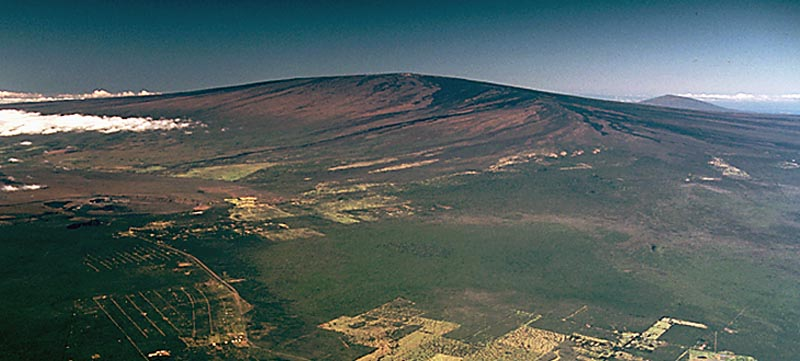
\includegraphics[width=0.8\linewidth]{images/book1/g7-mauna-loa.jpg}

{\small 从空中看到的夏威夷大岛盾状\omterm{def:g4:volcanoes-earthquakes-first-look:volcano}{火山}莫纳罗亚：
山体巨大、坡度平缓，由数千次流动性强的\omterm{def:g4:volcanoes-earthquakes-first-look:eruption}{熔岩}流堆积而成。
照片：J.~D. Griggs，U.S. Geological Survey，1985 年（公有
领域，经由维基共享资源）。}
% ledger: commons:mauna-loa
\label{fig:g7:volcanoes:mauna-loa}
\end{omfigure}

\section{与火山共处}

许多人住在\omterm{def:g4:volcanoes-earthquakes-first-look:volcano}{火山}附近：约 300 万人住在
1991 年皮纳图博\omterm{def:g4:volcanoes-earthquakes-first-look:volcano}{火山}周围的地区。幸运的是，大规模\omterm{def:g4:volcanoes-earthquakes-first-look:eruption}{喷发}往往会先发出
预兆。上升的\omterm{def:g7:volcanoes:magma}{岩浆}把\omterm{def:g3:stones-pebbles-sand:rock}{岩石}挤向一旁：地面开裂，
出现小\omterm{def:g4:volcanoes-earthquakes-first-look:earthquake}{地震}，山坡隆起，气体逸出。在圣海伦斯\omterm{def:g4:volcanoes-earthquakes-first-look:volcano}{火山}，
首次小\omterm{def:g4:volcanoes-earthquakes-first-look:earthquake}{地震}发生在 1980 年 3 月 16 日；至 5 月 17 日为止，
已记录到超过 10\,000 次\omterm{def:g4:volcanoes-earthquakes-first-look:earthquake}{地震}，北侧已向外鼓起
至少 \qty{137}{m}。科学家测量了这一切，该地区随即
被封闭。然而，仍有 57 人于 5 月 18 日遇难。
% ledger: usgs:msh-lead-up, usgs:msh-flows

1991 年，皮纳图博\omterm{def:g4:volcanoes-earthquakes-first-look:volcano}{火山}的科学家观察了\omterm{def:g4:volcanoes-earthquakes-first-look:earthquake}{地震}、气体
和\omterm{def:g4:volcanoes-earthquakes-first-look:volcano}{火山}隆起等迹象，及时发出了预警：住在\omterm{def:g4:volcanoes-earthquakes-first-look:volcano}{火山}附近的人
撤离了危险区，至少 5\,000 人的生命得以挽救。
% ledger: usgs:pinatubo-1991 (central Luzon home to about 3 million people)

\begin{remark}[切勿靠近正在喷发的火山]\label{rem:g7:volcanoes:safety}
观看\omterm{def:g4:volcanoes-earthquakes-first-look:volcano}{火山}\omterm{def:g4:volcanoes-earthquakes-first-look:eruption}{喷发}，只能在有关部门
开放的地点。气体、坠落的\omterm{def:g3:stones-pebbles-sand:rock}{岩石}、脚下会碎裂的新鲜\omterm{def:g4:volcanoes-earthquakes-first-look:eruption}{熔岩}壳
以及\omterm{def:g7:volcanoes:pyroclastic-flow}{火山碎屑流}，都可能致命，往往毫无预警。
\omterm{def:g4:volcanoes-earthquakes-first-look:volcano}{火山}观测站会公布哪些地点可以安全前往，务必遵守其指示。
\end{remark}

\section{练习}

\begin{exercise}[$\star$]\label{exo:g7:volcanoes:1}
请将下列词语与其含义配对：\omterm{def:g7:volcanoes:magma}{岩浆}、\omterm{def:g4:volcanoes-earthquakes-first-look:eruption}{熔岩}、\omterm{def:g7:volcanoes:magma-chamber}{岩浆房}、\omterm{def:g7:volcanoes:vent}{火山口通道}、
\omterm{def:g7:volcanoes:vent}{火山口}。(a) \omterm{def:g4:volcanoes-earthquakes-first-look:volcano}{火山}顶部碗状的凹陷。(b) 地下的熔融\omterm{def:g3:stones-pebbles-sand:rock}{岩石}。
(c) \omterm{def:g7:volcanoes:magma}{岩浆}喷出所经的开口。(d) 熔融的\omterm{def:g3:stones-pebbles-sand:rock}{岩石}
已经喷出地表。(e) \omterm{def:g4:volcanoes-earthquakes-first-look:volcano}{火山}下方几千米深处的大型
\omterm{def:g7:volcanoes:magma}{岩浆}囊。
\end{exercise}

\begin{exercise}[$\star$]\label{exo:g7:volcanoes:2}
溢流式还是爆炸式？(a) 炽热的\omterm{def:g4:volcanoes-earthquakes-first-look:eruption}{熔岩}河沿平缓的
山坡向下流动。(b) \omterm{def:g4:volcanoes-earthquakes-first-look:eruption}{火山灰}柱升入 \qty{35}{km} 高空。(c) 一
股炽热的熔滴从裂缝中喷出。(d) 热灰与气体组成的
炽热混合物沿\omterm{def:g1:landscapes-around-us:landform}{山谷}奔涌而下。
\end{exercise}

\begin{exercise}[$\star$]\label{exo:g7:volcanoes:3}
判断下列说法是否正确，并改正错误的说法。(a) \omterm{def:g7:volcanoes:magma}{岩浆}与\omterm{def:g4:volcanoes-earthquakes-first-look:eruption}{熔岩}是
同一种熔融\omterm{def:g3:stones-pebbles-sand:rock}{岩石}在地下与地表时的两个名称。(b) \omterm{def:g4:volcanoes-earthquakes-first-look:volcano}{火山}气体中最丰富的
是二氧化碳。(c) \omterm{def:g7:volcanoes:pyroclastic-flow}{火山碎屑流}是一条
液态\omterm{def:g4:volcanoes-earthquakes-first-look:eruption}{熔岩}\omterm{def:g1:landscapes-around-us:water}{河流}。(d) 夏威夷的\omterm{def:g4:volcanoes-earthquakes-first-look:volcano}{火山}位于\omterm{def:g7:plate-tectonics:plate-boundary}{板块边界}上。
\end{exercise}

\begin{exercise}[$\star$]\label{exo:g7:volcanoes:4}
利用发光颜色表。(a) \omterm{def:g4:volcanoes-earthquakes-first-look:eruption}{熔岩}发黄光，请给出其
温度。(b) 正在变硬的\omterm{def:g4:volcanoes-earthquakes-first-look:eruption}{熔岩}流发暗红色光，请给出其温度。
(c) 照片显示，\omterm{def:g4:volcanoes-earthquakes-first-look:eruption}{熔岩}流前缘为橙色，而
靠近\omterm{def:g7:volcanoes:vent}{火山口通道}处为黄色。哪一处温度更高？为什么？
\end{exercise}

\begin{exercise}[$\star\star$]\label{exo:g7:volcanoes:5}
利用 1\,214 座\omterm{def:g4:volcanoes-earthquakes-first-look:volcano}{火山}的柱状图。(a) 位于\omterm{def:g7:plate-tectonics:plate-boundary}{板块边界}上（即板块相互分离，或一个板块俯冲于
另一板块之下）的\omterm{def:g4:volcanoes-earthquakes-first-look:volcano}{火山}有多少座？
(b) 这些\omterm{def:g4:volcanoes-earthquakes-first-look:volcano}{火山}占全部\omterm{def:g4:volcanoes-earthquakes-first-look:volcano}{火山}的百分之几？(c) 核对
题中四个百分数之和约为 100~\%。
\end{exercise}

\begin{exercise}[$\star\star$]\label{exo:g7:volcanoes:6}
在所列的 660 座陡峭锥状\omterm{def:g4:volcanoes-earthquakes-first-look:volcano}{火山}（层状\omterm{def:g4:volcanoes-earthquakes-first-look:volcano}{火山}）中，564 座位于
一板块俯冲于另一板块之下处，62 座位于板块分离处，33 座位于
板块内部。(a) 求位于一板块俯冲于另一板块之下处的
陡峭锥状\omterm{def:g4:volcanoes-earthquakes-first-look:volcano}{火山}所占的百分比。(b) 剩下的陡峭锥状\omterm{def:g4:volcanoes-earthquakes-first-look:volcano}{火山}中，归入
“未知”的有多少座？(c) 利用四条线索判断，沿
环太平洋\omterm{def:g4:volcanoes-earthquakes-first-look:volcano}{火山}带应预期发生哪一类\omterm{def:g4:volcanoes-earthquakes-first-look:eruption}{喷发}？
\end{exercise}

\begin{exercise}[$\star\star$]\label{exo:g7:volcanoes:7}
基拉韦厄\omterm{def:g4:volcanoes-earthquakes-first-look:volcano}{火山}的\omterm{def:g4:volcanoes-earthquakes-first-look:eruption}{熔岩}离开\omterm{def:g7:volcanoes:vent}{火山口通道}时，温度约为 \qty{1170}{\degreeCelsius}；
在一条\omterm{def:g4:volcanoes-earthquakes-first-look:eruption}{熔岩}隧道中，\omterm{def:g4:volcanoes-earthquakes-first-look:eruption}{熔岩}流到 \qty{10}{km} 外的海边，温度约为
\qty{1140}{\degreeCelsius}。(a) \omterm{def:g4:volcanoes-earthquakes-first-look:eruption}{熔岩}降温了多少度？(b) 每千米降温
多少度？(c) 露天\omterm{def:g4:volcanoes-earthquakes-first-look:eruption}{熔岩}的表面每秒降温
可达数百度。试解释隧道中的\omterm{def:g4:volcanoes-earthquakes-first-look:eruption}{熔岩}
为何仍能保持如此高温。
\end{exercise}

\begin{exercise}[$\star\star$]\label{exo:g7:volcanoes:8}
考爱岛上最古老的\omterm{def:g3:stones-pebbles-sand:rock}{岩石}约 550 万年；大岛
的\omterm{def:g3:stones-pebbles-sand:rock}{岩石}不到 70 万年。(a) 哪个岛更古老？至少古老
多少百万年？(b) 哪个岛被\omterm{def:g5:water-shapes-the-land:erosion}{侵蚀}得更厉害？为什么？
(c) 今天哪个岛位于\omterm{def:g7:volcanoes:hotspot}{热点}之上？(d) 考爱岛位于
大岛的西北方。太平洋板块将这些岛屿
向哪个方向搬运？
\end{exercise}

\begin{exercise}[$\star\star$]\label{exo:g7:volcanoes:9}
夏威夷群岛距离最近的\omterm{def:g7:plate-tectonics:plate-boundary}{板块边界}超过 \qty{3200}{km}。
(a) 这对\omterm{def:g4:volcanoes-earthquakes-first-look:volcano}{火山}而言为何令人意外？(b) 用三到四句话说明
其\omterm{def:g7:volcanoes:magma}{岩浆}来自何处。(c) 在\omterm{def:g4:volcanoes-earthquakes-first-look:volcano}{火山}分布图上，
它们是什么颜色？
\end{exercise}

\begin{exercise}[$\star\star$]\label{exo:g7:volcanoes:10}
1991 年 6 月，皮纳图博\omterm{def:g4:volcanoes-earthquakes-first-look:volcano}{火山}最初的\omterm{def:g7:volcanoes:magma}{岩浆}悄然渗出；三天
后，另一批\omterm{def:g7:volcanoes:magma}{岩浆}爆发了。利用两瓶汽水，解释
这一差异。两批\omterm{def:g7:volcanoes:magma}{岩浆}中，哪一批在上升途中已经失去了气体？
\end{exercise}

\begin{exercise}[$\star\star\star$]\label{exo:g7:volcanoes:11}
一座村庄位于\omterm{def:g4:volcanoes-earthquakes-first-look:volcano}{火山}下游的\omterm{def:g1:landscapes-around-us:landform}{山谷}中，距\omterm{def:g4:volcanoes-earthquakes-first-look:volcano}{火山} \qty{10}{km}。（a）
\omterm{def:g7:volcanoes:pyroclastic-flow}{火山碎屑流}以 \qty{80}{km/h} 的速度运动，它需要多少分钟才能到达村庄？
（b）若速度为 \qty{130}{km/h}，问题相同。（c）一户人家乘车撤离
需要 20~分钟。试说明为何预警必须在\omterm{def:g4:volcanoes-earthquakes-first-look:eruption}{喷发}开始之前发出，
而不是等到看见\omterm{def:g7:volcanoes:pyroclastic-flow}{火山碎屑流}时才发出。
\end{exercise}

\begin{exercise}[$\star\star\star$]\label{exo:g7:volcanoes:12}
圣海伦\omterm{def:g4:volcanoes-earthquakes-first-look:volcano}{火山}喷出的\omterm{def:g4:volcanoes-earthquakes-first-look:eruption}{火山灰}在 15~天内绕地球一周。
\omterm{def:g6:latitude-longitude:latitude}{纬度}每度约 \qty{111}{km}，一整圈为
360~度。（a）地球一整圈约长多少千米？
结果取最接近的千位数。（b）
\omterm{def:g4:volcanoes-earthquakes-first-look:eruption}{火山灰}平均每天移动多少千米？（c）这相当于每小时多少千米？
（d）\omterm{def:g4:volcanoes-earthquakes-first-look:eruption}{火山灰}是被风带动的，还是依靠自身速度运动的？请说明理由。
% ledger: usgs:msh-may18, rmg:latitude-def
\end{exercise}

\section{问题：山峰失去山顶的那一天}

\begin{problem}[{周末问题——圣海伦火山的预警迹象，
1980 年 5 月 18 日的喷发，以及山体损失了多少}]
\label{pb:g7:volcanoes:1}
% ledger: usgs:msh-heights, usgs:msh-lead-up, usgs:msh-may18, usgs:msh-flows, usgs:msh-reach, usgs:msh-dome, usgs:msh-faq-loss, data:gvp, tht:everest

圣海伦\omterm{def:g4:volcanoes-earthquakes-first-look:volcano}{火山}位于美国西北部。请结合
本章开头的照片、\omterm{def:g4:volcanoes-earthquakes-first-look:volcano}{火山}分布图以及
下面的数据作答，这些数据由美国地质调查局测得。

\medskip
\noindent\textbf{第一部分——\omterm{def:g4:volcanoes-earthquakes-first-look:eruption}{喷发}之前。}
\begin{enumerate}
  \item 1980 年 3 月 16 日出现了最初的小\omterm{def:g4:volcanoes-earthquakes-first-look:earthquake}{地震}，
        5 月 18 日发生了大规模\omterm{def:g4:volcanoes-earthquakes-first-look:eruption}{喷发}。两者之间相隔多少天？（3 月有 31 天，
        4 月有 30 天。）
  \item 到 5 月 17 日，已记录到超过 10\,000 次\omterm{def:g4:volcanoes-earthquakes-first-look:earthquake}{地震}，
        自 3 月 16 日以来的 62~天里，
        平均每天约有多少次？
  \item 山体北侧向外隆起了至少
        \qty{137}{m}。试说明这种隆起为何令科学家担忧。
  \item 在\omterm{def:g4:volcanoes-earthquakes-first-look:volcano}{火山}分布图上，圣海伦\omterm{def:g4:volcanoes-earthquakes-first-look:volcano}{火山}用一个蓝色三角形表示。
        这说明它处于怎样的构造环境中？你预计它会发生哪一类\omterm{def:g4:volcanoes-earthquakes-first-look:eruption}{喷发}，
        又会形成哪种形状的\omterm{def:g4:volcanoes-earthquakes-first-look:volcano}{火山}？
\end{enumerate}

\medskip
\noindent\textbf{第二部分——1980 年 5 月 18 日。}\par\nopagebreak
\begin{enumerate}[resume, beginpenalty=10000]
  \item 8:32 时，一次小\omterm{def:g4:volcanoes-earthquakes-first-look:earthquake}{地震}使隆起的一侧开始滑动。
        \omterm{def:g5:natural-hazards:landslide}{滑坡}的速度最高达 \qty{240}{km/h}，
        这相当于每分钟多少千米？
  \item \omterm{def:g5:natural-hazards:landslide}{滑坡}使\omterm{def:g7:volcanoes:magma}{岩浆}暴露出来，如同摇晃后的瓶子被拔开了瓶塞。
        试说明\omterm{def:g4:volcanoes-earthquakes-first-look:volcano}{火山}为何随后向侧面爆发。
  \item 侧向爆发的速度至少为 \qty{480}{km/h}，并
        到达距\omterm{def:g4:volcanoes-earthquakes-first-look:volcano}{火山} \qty{27}{km} 处。以此速度计算，
        最多需要多少分钟才能到达那里？
  \item \omterm{def:g7:volcanoes:pyroclastic-flow}{火山碎屑流}的速度最高达 \qty{130}{km/h}，并到达距\omterm{def:g7:volcanoes:vent}{火山口}
        \qty{8}{km} 处。以此速度计算，它们需要多少分钟？
        结果取最接近的整数分钟。
\end{enumerate}

\medskip
\noindent\textbf{第三部分——\omterm{def:g4:volcanoes-earthquakes-first-look:eruption}{喷发}之后。}\par\nopagebreak
\begin{enumerate}[resume, beginpenalty=10000]
  \item \omterm{def:g4:volcanoes-earthquakes-first-look:eruption}{火山灰}柱在不到
        15~分钟内升至约 \qty{24}{km} 的高度。这相当于珠穆朗玛峰
        （\qty{8.8}{km}）的多少倍？结果保留一位小数。
  \item 1980 至 1986 年间，黏稠的\omterm{def:g4:volcanoes-earthquakes-first-look:eruption}{熔岩}在\omterm{def:g7:volcanoes:vent}{火山口}溢出，
        并在\omterm{def:g7:volcanoes:vent}{火山口通道}上方堆起了高 \qty{267}{m} 的土丘。这些\omterm{def:g4:volcanoes-earthquakes-first-look:eruption}{喷发}
        是溢流式的还是爆炸式的？它们让你想起了
        哪一瓶汽水？
  \item 观察\omterm{def:g4:volcanoes-earthquakes-first-look:volcano}{火山}的两张照片，用两句话描述
        发生了什么变化。
  \item \omterm{def:g4:volcanoes-earthquakes-first-look:eruption}{喷发}前，山顶\omterm{def:g4:world-physical-map:altitude}{海拔}为 \qty{2950}{m}；
        \omterm{def:g4:volcanoes-earthquakes-first-look:eruption}{喷发}后，最高点为 \qty{2549}{m}。
        山体高度减少了多少米？
\end{enumerate}
\end{problem}
